\documentclass[border=2pt]{standalone}
\usepackage{amsmath, amsthm, amsfonts}
\usepackage{tikz-cd, kotex}
\usepackage{quiver}
\usepackage{Operators}
\usepackage{palette}
\usepackage{diagram-style}
\begin{document}

%%FIG parallelepiped (Determinant-1.svg)
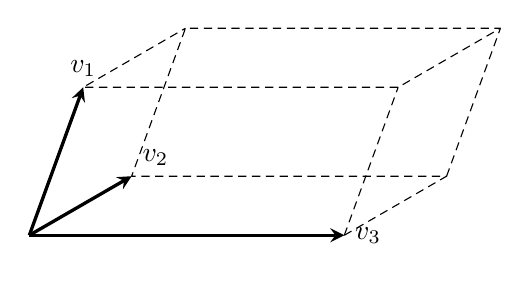
\begin{tikzpicture}
	\begin{scope}[x={(4cm,0cm)},y={({cos(30)*1.5cm},{sin(30)*1.5cm})},z={({cos(70)*2cm},{sin(70)*2cm})},line join=round]
		\draw[densely dashed] (1,0,0) -- (1,1,0) -- (0,1,0) -- (0,1,1) -- (1,1,1) -- (1,0,1) -- (0,0,1) -- (0,1,1);
		\draw[densely dashed] (1,0,0) -- (1,0,1);
		\draw[densely dashed] (1,1,0) -- (1,1,1);
		\draw[very thick, -{stealth}, black] (0,0,0)--(0,0,1) node[above]{$v_1$};
		\draw[very thick, -{stealth}, black] (0,0,0)--(0,1,0) node[above right]{$v_2$};
		\draw[very thick, -{stealth}, black] (0,0,0)--(1,0,0) node[right]{$v_3$};
	\end{scope}
\end{tikzpicture}

%%FIG Square (Determinant-2.svg)
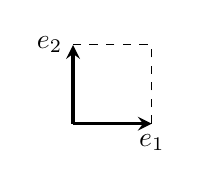
\begin{tikzpicture}
\draw[very thick, -{stealth}] (0,0)--(0,1) node[left]{$e_2$};
\draw[very thick, -{stealth}] (0,0)--(1,0) node[below]{$e_1$};
\draw[dashed] (1,0)--(1,1)--(0,1);
\end{tikzpicture}

%%FIG Transformation (Determinant-3.svg)
\begin{tikzpicture}
\draw[ -{stealth}] (0,0)--(0.5,1);
\draw[very thin,densely dotted] (0,0)--(1,0)--(1.5,1)--(0.5,1)--cycle;
\draw[thick, accent1, -{stealth}] (0,0)--(1,1) node[above]{};
\draw[thick, accent1, -{stealth}] (0,0)--(1,0) node[below]{};
\draw[accent1, loosely dashed] (1,1)--(2,1)--(1,0);
\fill[accent1, opacity=.2] (0,0)--(1,0)--(2,1)--(1,1)--cycle;
\draw[thin, black!50, -{stealth}] (0.5,1)--(1,1);
\end{tikzpicture}
\hspace{10pt}
\begin{tikzpicture}
\filldraw[densely dotted, fill=black!20] (0,0)--(1,0)--(1.5,1)--(.5,1)--cycle;
\draw[thick, -{stealth}] (0,0)--(1,0);
\draw[thick, -{stealth}] (0,0)--(.5,1);
\draw[loosely dashed, accent1] (.5,1)--(2.5,1)--(2,0);
\fill[accent1!20] (1,0)--(2,0)--(2.5,1)--(1.5,1)--cycle;
\draw[accent1, -{stealth}] (0,0)--(2,0) node[below]{};
\end{tikzpicture}

%%FIG Multilinearity (Determinant-4.svg)
\begin{tikzpicture}
	\draw[thick, black!50, -{stealth}] (0,0)--(1,0) node[below]{};
	\draw[thick, black!50, -{stealth}] (0,0)--(1,1);
	\draw[thick, black!50, -{stealth}] (1,1)--(1.5,2) node[above]{};
	\draw[black!50, densely dotted] (1,1)--(2,1)--(1,0);
	\draw[black!50, densely dotted] (1.5,2)--(2.5,2)--(2,1);
	\draw[black!50, thick, -{stealth}] (1,1)--(2,1);
	\draw[thick, accent1, -{stealth}] (0,0)--(1.5,2);
	\draw[thick, dashed, accent1] (1,0)--(2.5,2);
	\fill[accent1, opacity=.2] (0,0)--(1,0)--(2.5,2)--(1.5,2)--cycle;
\end{tikzpicture}

\end{document}
